\documentclass[1p]{elsarticle_modified}
%\bibliographystyle{elsarticle-num}

%\usepackage[colorlinks]{hyperref}
%\usepackage{abbrmath_seonhwa} %\Abb, \Ascr, \Acal ,\Abf, \Afrak
\usepackage{amsfonts}
\usepackage{amssymb}
\usepackage{amsmath}
\usepackage{amsthm}
\usepackage{scalefnt}
\usepackage{amsbsy}
\usepackage{kotex}
\usepackage{caption}
\usepackage{subfig}
\usepackage{color}
\usepackage{graphicx}
\usepackage{xcolor} %% white, black, red, green, blue, cyan, magenta, yellow
\usepackage{float}
\usepackage{setspace}
\usepackage{hyperref}

\usepackage{tikz}
\usetikzlibrary{arrows}

\usepackage{multirow}
\usepackage{array} % fixed length table
\usepackage{hhline}

%%%%%%%%%%%%%%%%%%%%%
\makeatletter
\renewcommand*\env@matrix[1][\arraystretch]{%
	\edef\arraystretch{#1}%
	\hskip -\arraycolsep
	\let\@ifnextchar\new@ifnextchar
	\array{*\c@MaxMatrixCols c}}
\makeatother %https://tex.stackexchange.com/questions/14071/how-can-i-increase-the-line-spacing-in-a-matrix
%%%%%%%%%%%%%%%

\usepackage[normalem]{ulem}

\newcommand{\msout}[1]{\ifmmode\text{\sout{\ensuremath{#1}}}\else\sout{#1}\fi}
%SOURCE: \msout is \stkout macro in https://tex.stackexchange.com/questions/20609/strikeout-in-math-mode

\newcommand{\cancel}[1]{
	\ifmmode
	{\color{red}\msout{#1}}
	\else
	{\color{red}\sout{#1}}
	\fi
}

\newcommand{\add}[1]{
	{\color{blue}\uwave{#1}}
}

\newcommand{\replace}[2]{
	\ifmmode
	{\color{red}\msout{#1}}{\color{blue}\uwave{#2}}
	\else
	{\color{red}\sout{#1}}{\color{blue}\uwave{#2}}
	\fi
}

\newcommand{\Sol}{\mathcal{S}} %segment
\newcommand{\D}{D} %diagram
\newcommand{\A}{\mathcal{A}} %arc


%%%%%%%%%%%%%%%%%%%%%%%%%%%%%5 test

\def\sl{\operatorname{\textup{SL}}(2,\Cbb)}
\def\psl{\operatorname{\textup{PSL}}(2,\Cbb)}
\def\quan{\mkern 1mu \triangleright \mkern 1mu}

\theoremstyle{definition}
\newtheorem{thm}{Theorem}[section]
\newtheorem{prop}[thm]{Proposition}
\newtheorem{lem}[thm]{Lemma}
\newtheorem{ques}[thm]{Question}
\newtheorem{cor}[thm]{Corollary}
\newtheorem{defn}[thm]{Definition}
\newtheorem{exam}[thm]{Example}
\newtheorem{rmk}[thm]{Remark}
\newtheorem{alg}[thm]{Algorithm}

\newcommand{\I}{\sqrt{-1}}
\begin{document}

%\begin{frontmatter}
%
%\title{Boundary parabolic representations of knots up to 8 crossings}
%
%%% Group authors per affiliation:
%\author{Yunhi Cho} 
%\address{Department of Mathematics, University of Seoul, Seoul, Korea}
%\ead{yhcho@uos.ac.kr}
%
%
%\author{Seonhwa Kim} %\fnref{s_kim}}
%\address{Center for Geometry and Physics, Institute for Basic Science, Pohang, 37673, Korea}
%\ead{ryeona17@ibs.re.kr}
%
%\author{Hyuk Kim}
%\address{Department of Mathematical Sciences, Seoul National University, Seoul 08826, Korea}
%\ead{hyukkim@snu.ac.kr}
%
%\author{Seokbeom Yoon}
%\address{Department of Mathematical Sciences, Seoul National University, Seoul, 08826,  Korea}
%\ead{sbyoon15@snu.ac.kr}
%
%\begin{abstract}
%We find all boundary parabolic representation of knots up to 8 crossings.
%
%\end{abstract}
%\begin{keyword}
%    \MSC[2010] 57M25 
%\end{keyword}
%
%\end{frontmatter}

%\linenumbers
%\tableofcontents
%
\newcommand\colored[1]{\textcolor{white}{\rule[-0.35ex]{0.8em}{1.4ex}}\kern-0.8em\color{red} #1}%
%\newcommand\colored[1]{\textcolor{white}{ #1}\kern-2.17ex	\textcolor{white}{ #1}\kern-1.81ex	\textcolor{white}{ #1}\kern-2.15ex\color{red}#1	}

{\Large $\underline{12n_{0152}~(K12n_{0152})}$}

\setlength{\tabcolsep}{10pt}
\renewcommand{\arraystretch}{1.6}
\vspace{1cm}\begin{tabular}{m{100pt}>{\centering\arraybackslash}m{274pt}}
\multirow{5}{120pt}{
	\centering
	\includegraphics[width=112pt]{../../../GIT/diagram.site/Diagrams/png/2241_12n_0152.png}\\
\ \ \ A knot diagram\footnotemark}&
\allowdisplaybreaks
\textbf{Linearized knot diagam} \\
\cline{2-2}
 &
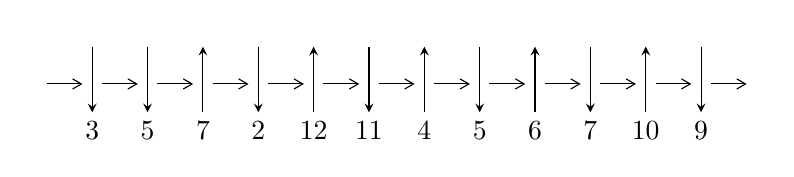
\begin{tikzpicture}[x=20pt, y=17pt]
	% nodes
	\node (C0) at (0, 0) {};
	\node (C1) at (1, 0) {};
	\node (C1U) at (1, +1) {};
	\node (C1D) at (1, -1) {3};

	\node (C2) at (2, 0) {};
	\node (C2U) at (2, +1) {};
	\node (C2D) at (2, -1) {5};

	\node (C3) at (3, 0) {};
	\node (C3U) at (3, +1) {};
	\node (C3D) at (3, -1) {7};

	\node (C4) at (4, 0) {};
	\node (C4U) at (4, +1) {};
	\node (C4D) at (4, -1) {2};

	\node (C5) at (5, 0) {};
	\node (C5U) at (5, +1) {};
	\node (C5D) at (5, -1) {12};

	\node (C6) at (6, 0) {};
	\node (C6U) at (6, +1) {};
	\node (C6D) at (6, -1) {11};

	\node (C7) at (7, 0) {};
	\node (C7U) at (7, +1) {};
	\node (C7D) at (7, -1) {4};

	\node (C8) at (8, 0) {};
	\node (C8U) at (8, +1) {};
	\node (C8D) at (8, -1) {5};

	\node (C9) at (9, 0) {};
	\node (C9U) at (9, +1) {};
	\node (C9D) at (9, -1) {6};

	\node (C10) at (10, 0) {};
	\node (C10U) at (10, +1) {};
	\node (C10D) at (10, -1) {7};

	\node (C11) at (11, 0) {};
	\node (C11U) at (11, +1) {};
	\node (C11D) at (11, -1) {10};

	\node (C12) at (12, 0) {};
	\node (C12U) at (12, +1) {};
	\node (C12D) at (12, -1) {9};
	\node (C13) at (13, 0) {};

	% arrows
	\draw[->,>={angle 60}]
	(C0) edge (C1) (C1) edge (C2) (C2) edge (C3) (C3) edge (C4) (C4) edge (C5) (C5) edge (C6) (C6) edge (C7) (C7) edge (C8) (C8) edge (C9) (C9) edge (C10) (C10) edge (C11) (C11) edge (C12) (C12) edge (C13) ;	\draw[->,>=stealth]
	(C1U) edge (C1D) (C2U) edge (C2D) (C3D) edge (C3U) (C4U) edge (C4D) (C5D) edge (C5U) (C6U) edge (C6D) (C7D) edge (C7U) (C8U) edge (C8D) (C9D) edge (C9U) (C10U) edge (C10D) (C11D) edge (C11U) (C12U) edge (C12D) ;
	\end{tikzpicture} \\
\hhline{~~} \\& 
\textbf{Solving Sequence} \\ \cline{2-2} 
 &
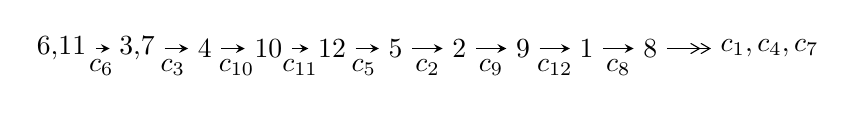
\begin{tikzpicture}[x=23pt, y=7pt]
	% node
	\node (A0) at (-1/8, 0) {6,11};
	\node (A1) at (17/16, 0) {3,7};
	\node (A2) at (17/8, 0) {4};
	\node (A3) at (25/8, 0) {10};
	\node (A4) at (33/8, 0) {12};
	\node (A5) at (41/8, 0) {5};
	\node (A6) at (49/8, 0) {2};
	\node (A7) at (57/8, 0) {9};
	\node (A8) at (65/8, 0) {1};
	\node (A9) at (73/8, 0) {8};
	\node (C1) at (1/2, -1) {$c_{6}$};
	\node (C2) at (13/8, -1) {$c_{3}$};
	\node (C3) at (21/8, -1) {$c_{10}$};
	\node (C4) at (29/8, -1) {$c_{11}$};
	\node (C5) at (37/8, -1) {$c_{5}$};
	\node (C6) at (45/8, -1) {$c_{2}$};
	\node (C7) at (53/8, -1) {$c_{9}$};
	\node (C8) at (61/8, -1) {$c_{12}$};
	\node (C9) at (69/8, -1) {$c_{8}$};
	\node (A10) at (11, 0) {$c_{1},c_{4},c_{7}$};

	% edge
	\draw[->,>=stealth]	
	(A0) edge (A1) (A1) edge (A2) (A2) edge (A3) (A3) edge (A4) (A4) edge (A5) (A5) edge (A6) (A6) edge (A7) (A7) edge (A8) (A8) edge (A9) ;
	\draw[->>,>={angle 60}]	
	(A9) edge (A10);
\end{tikzpicture} \\ 

\end{tabular} \\

\footnotetext{
The image of knot diagram is generated by the software ``\textbf{Draw programme}" developed by Andrew Bartholomew(\url{http://www.layer8.co.uk/maths/draw/index.htm\#Running-draw}), where we modified some parts for our purpose(\url{https://github.com/CATsTAILs/LinksPainter}).
}\phantom \\ \newline 
\centering \textbf{Ideals for irreducible components\footnotemark of $X_{\text{par}}$} 
 
\begin{align*}
I^u_{1}&=\langle 
u^{42}- u^{41}+\cdots- u^3+b,\;- u^{42}+u^{41}+\cdots+a-1,\;u^{44}-2 u^{43}+\cdots-2 u+1\rangle \\
I^u_{2}&=\langle 
b+u,\;- u^3+a- u+1,\;u^4+u^2- u+1\rangle \\
I^u_{3}&=\langle 
- u^5- u^4-2 u^3-2 u^2+b-2 u-1,\;u^4+u^2+a,\;u^6+u^5+2 u^4+2 u^3+2 u^2+2 u+1\rangle \\
\\
\end{align*}
\raggedright * 3 irreducible components of $\dim_{\mathbb{C}}=0$, with total 54 representations.\\
\footnotetext{All coefficients of polynomials are rational numbers. But the coefficients are sometimes approximated in decimal forms when there is not enough margin.}
\newpage
\renewcommand{\arraystretch}{1}
\centering \section*{I. $I^u_{1}= \langle u^{42}- u^{41}+\cdots- u^3+b,\;- u^{42}+u^{41}+\cdots+a-1,\;u^{44}-2 u^{43}+\cdots-2 u+1 \rangle$}
\flushleft \textbf{(i) Arc colorings}\\
\begin{tabular}{m{7pt} m{180pt} m{7pt} m{180pt} }
\flushright $a_{6}=$&$\begin{pmatrix}1\\0\end{pmatrix}$ \\
\flushright $a_{11}=$&$\begin{pmatrix}0\\u\end{pmatrix}$ \\
\flushright $a_{3}=$&$\begin{pmatrix}u^{42}- u^{41}+\cdots+4 u^3+1\\- u^{42}+u^{41}+\cdots-5 u^4+u^3\end{pmatrix}$ \\
\flushright $a_{7}=$&$\begin{pmatrix}1\\u^2\end{pmatrix}$ \\
\flushright $a_{4}=$&$\begin{pmatrix}- u^{43}+3 u^{42}+\cdots-2 u+2\\u^{43}-3 u^{42}+\cdots- u^2+u\end{pmatrix}$ \\
\flushright $a_{10}=$&$\begin{pmatrix}u\\u^3+u\end{pmatrix}$ \\
\flushright $a_{12}=$&$\begin{pmatrix}u^3\\u^5+u^3+u\end{pmatrix}$ \\
\flushright $a_{5}=$&$\begin{pmatrix}u^8+u^6+u^4+1\\u^{10}+2 u^8+3 u^6+2 u^4+u^2\end{pmatrix}$ \\
\flushright $a_{2}=$&$\begin{pmatrix}u^{39}- u^{38}+\cdots+u+1\\u^{41}- u^{40}+\cdots+u^3+u^2\end{pmatrix}$ \\
\flushright $a_{9}=$&$\begin{pmatrix}- u^3\\u^3+u\end{pmatrix}$ \\
\flushright $a_{1}=$&$\begin{pmatrix}- u^{11}-2 u^9-2 u^7+u^3\\u^{11}+3 u^9+4 u^7+3 u^5+u^3+u\end{pmatrix}$ \\
\flushright $a_{8}=$&$\begin{pmatrix}u^{21}+4 u^{19}+9 u^{17}+12 u^{15}+12 u^{13}+10 u^{11}+9 u^9+6 u^7+3 u^5+u\\u^{23}+5 u^{21}+\cdots+2 u^3+u\end{pmatrix}$\\&\end{tabular}
\flushleft \textbf{(ii) Obstruction class $= -1$}\\~\\
\flushleft \textbf{(iii) Cusp Shapes $= 4 u^{43}-8 u^{42}+\cdots+11 u-10$}\\~\\
\newpage\renewcommand{\arraystretch}{1}
\flushleft \textbf{(iv) u-Polynomials at the component}\newline \\
\begin{tabular}{m{50pt}|m{274pt}}
Crossings & \hspace{64pt}u-Polynomials at each crossing \\
\hline $$\begin{aligned}c_{1}\end{aligned}$$&$\begin{aligned}
&u^{44}+5 u^{43}+\cdots+5 u+1
\end{aligned}$\\
\hline $$\begin{aligned}c_{2},c_{4}\end{aligned}$$&$\begin{aligned}
&u^{44}-11 u^{43}+\cdots-9 u+1
\end{aligned}$\\
\hline $$\begin{aligned}c_{3},c_{7}\end{aligned}$$&$\begin{aligned}
&u^{44}- u^{43}+\cdots-2048 u+1024
\end{aligned}$\\
\hline $$\begin{aligned}c_{5}\end{aligned}$$&$\begin{aligned}
&u^{44}+10 u^{43}+\cdots+510 u+61
\end{aligned}$\\
\hline $$\begin{aligned}c_{6},c_{10}\end{aligned}$$&$\begin{aligned}
&u^{44}+2 u^{43}+\cdots+2 u+1
\end{aligned}$\\
\hline $$\begin{aligned}c_{8}\end{aligned}$$&$\begin{aligned}
&u^{44}+2 u^{43}+\cdots-12568908 u+4045417
\end{aligned}$\\
\hline $$\begin{aligned}c_{9}\end{aligned}$$&$\begin{aligned}
&u^{44}-2 u^{43}+\cdots-48 u+72
\end{aligned}$\\
\hline $$\begin{aligned}c_{11}\end{aligned}$$&$\begin{aligned}
&u^{44}-22 u^{43}+\cdots-2 u+1
\end{aligned}$\\
\hline $$\begin{aligned}c_{12}\end{aligned}$$&$\begin{aligned}
&u^{44}-2 u^{43}+\cdots-2 u+1
\end{aligned}$\\
\hline
\end{tabular}\\~\\
\newpage\renewcommand{\arraystretch}{1}
\flushleft \textbf{(v) Riley Polynomials at the component}\newline \\
\begin{tabular}{m{50pt}|m{274pt}}
Crossings & \hspace{64pt}Riley Polynomials at each crossing \\
\hline $$\begin{aligned}c_{1}\end{aligned}$$&$\begin{aligned}
&y^{44}+79 y^{43}+\cdots+63 y+1
\end{aligned}$\\
\hline $$\begin{aligned}c_{2},c_{4}\end{aligned}$$&$\begin{aligned}
&y^{44}-5 y^{43}+\cdots-5 y+1
\end{aligned}$\\
\hline $$\begin{aligned}c_{3},c_{7}\end{aligned}$$&$\begin{aligned}
&y^{44}-63 y^{43}+\cdots-17301504 y+1048576
\end{aligned}$\\
\hline $$\begin{aligned}c_{5}\end{aligned}$$&$\begin{aligned}
&y^{44}-10 y^{43}+\cdots+42582 y+3721
\end{aligned}$\\
\hline $$\begin{aligned}c_{6},c_{10}\end{aligned}$$&$\begin{aligned}
&y^{44}+22 y^{43}+\cdots+2 y+1
\end{aligned}$\\
\hline $$\begin{aligned}c_{8}\end{aligned}$$&$\begin{aligned}
&y^{44}+118 y^{43}+\cdots+59158715268238 y+16365398703889
\end{aligned}$\\
\hline $$\begin{aligned}c_{9}\end{aligned}$$&$\begin{aligned}
&y^{44}-18 y^{43}+\cdots-39312 y+5184
\end{aligned}$\\
\hline $$\begin{aligned}c_{11}\end{aligned}$$&$\begin{aligned}
&y^{44}+2 y^{43}+\cdots+22 y+1
\end{aligned}$\\
\hline $$\begin{aligned}c_{12}\end{aligned}$$&$\begin{aligned}
&y^{44}+58 y^{43}+\cdots+2 y+1
\end{aligned}$\\
\hline
\end{tabular}\\~\\
\newpage\flushleft \textbf{(vi) Complex Volumes and Cusp Shapes}
$$\begin{array}{c|c|c}  
\text{Solutions to }I^u_{1}& \I (\text{vol} + \sqrt{-1}CS) & \text{Cusp shape}\\
 \hline 
\begin{aligned}
u &= -0.650835 + 0.753787 I \\
a &= \phantom{-}0.08846 - 1.78587 I \\
b &= \phantom{-}0.081004 + 0.538151 I\end{aligned}
 & \phantom{-}7.53342 + 6.30806 I & -1.89413 - 5.29683 I \\ \hline\begin{aligned}
u &= -0.650835 - 0.753787 I \\
a &= \phantom{-}0.08846 + 1.78587 I \\
b &= \phantom{-}0.081004 - 0.538151 I\end{aligned}
 & \phantom{-}7.53342 - 6.30806 I & -1.89413 + 5.29683 I \\ \hline\begin{aligned}
u &= -0.632673 + 0.802636 I \\
a &= \phantom{-}0.267451 + 1.071980 I \\
b &= -0.836036 - 0.256227 I\end{aligned}
 & \phantom{-}7.68178 - 1.36168 I & -1.47660 - 0.85903 I \\ \hline\begin{aligned}
u &= -0.632673 - 0.802636 I \\
a &= \phantom{-}0.267451 - 1.071980 I \\
b &= -0.836036 + 0.256227 I\end{aligned}
 & \phantom{-}7.68178 + 1.36168 I & -1.47660 + 0.85903 I \\ \hline\begin{aligned}
u &= \phantom{-}0.524889 + 0.986478 I \\
a &= \phantom{-}0.205755 - 0.498882 I \\
b &= -0.239518 + 0.643052 I\end{aligned}
 & -0.15574 - 2.57093 I & \phantom{-}0.70156 + 2.32156 I \\ \hline\begin{aligned}
u &= \phantom{-}0.524889 - 0.986478 I \\
a &= \phantom{-}0.205755 + 0.498882 I \\
b &= -0.239518 - 0.643052 I\end{aligned}
 & -0.15574 + 2.57093 I & \phantom{-}0.70156 - 2.32156 I \\ \hline\begin{aligned}
u &= -0.238245 + 1.098530 I \\
a &= -1.052800 - 0.393118 I \\
b &= \phantom{-}0.056688 + 0.785185 I\end{aligned}
 & \phantom{-}4.15035 - 1.19914 I & \phantom{-}5.43856 + 1.99279 I \\ \hline\begin{aligned}
u &= -0.238245 - 1.098530 I \\
a &= -1.052800 + 0.393118 I \\
b &= \phantom{-}0.056688 - 0.785185 I\end{aligned}
 & \phantom{-}4.15035 + 1.19914 I & \phantom{-}5.43856 - 1.99279 I \\ \hline\begin{aligned}
u &= \phantom{-}0.401111 + 1.053070 I \\
a &= -0.924275 - 0.254329 I \\
b &= \phantom{-}0.940261 + 0.336917 I\end{aligned}
 & \phantom{-}1.12314 - 1.53132 I & \phantom{-}0.534904 + 0.918296 I \\ \hline\begin{aligned}
u &= \phantom{-}0.401111 - 1.053070 I \\
a &= -0.924275 + 0.254329 I \\
b &= \phantom{-}0.940261 - 0.336917 I\end{aligned}
 & \phantom{-}1.12314 + 1.53132 I & \phantom{-}0.534904 - 0.918296 I\\
 \hline 
 \end{array}$$\newpage$$\begin{array}{c|c|c}  
\text{Solutions to }I^u_{1}& \I (\text{vol} + \sqrt{-1}CS) & \text{Cusp shape}\\
 \hline 
\begin{aligned}
u &= \phantom{-}0.806426 + 0.270607 I \\
a &= \phantom{-}0.528240 - 1.204320 I \\
b &= \phantom{-}2.74166 + 0.03423 I\end{aligned}
 & \phantom{-}10.03900 + 8.32938 I & -1.08270 - 4.13842 I \\ \hline\begin{aligned}
u &= \phantom{-}0.806426 - 0.270607 I \\
a &= \phantom{-}0.528240 + 1.204320 I \\
b &= \phantom{-}2.74166 - 0.03423 I\end{aligned}
 & \phantom{-}10.03900 - 8.32938 I & -1.08270 + 4.13842 I \\ \hline\begin{aligned}
u &= \phantom{-}0.605593 + 0.584352 I \\
a &= -0.793404 + 0.445925 I \\
b &= \phantom{-}0.360026 - 0.418150 I\end{aligned}
 & -1.33551 - 1.91461 I & -1.93635 + 4.43568 I \\ \hline\begin{aligned}
u &= \phantom{-}0.605593 - 0.584352 I \\
a &= -0.793404 - 0.445925 I \\
b &= \phantom{-}0.360026 + 0.418150 I\end{aligned}
 & -1.33551 + 1.91461 I & -1.93635 - 4.43568 I \\ \hline\begin{aligned}
u &= -0.470021 + 1.059020 I \\
a &= -2.48227 + 1.10683 I \\
b &= \phantom{-}2.56335 + 1.29163 I\end{aligned}
 & -0.51801 + 3.33956 I & \phantom{-}1.74785 - 5.30450 I \\ \hline\begin{aligned}
u &= -0.470021 - 1.059020 I \\
a &= -2.48227 - 1.10683 I \\
b &= \phantom{-}2.56335 - 1.29163 I\end{aligned}
 & -0.51801 - 3.33956 I & \phantom{-}1.74785 + 5.30450 I \\ \hline\begin{aligned}
u &= \phantom{-}0.801520 + 0.234624 I \\
a &= -0.402454 + 0.655071 I \\
b &= -2.50289 + 0.41075 I\end{aligned}
 & \phantom{-}10.56280 + 0.28731 I & -0.340463 + 0.065100 I \\ \hline\begin{aligned}
u &= \phantom{-}0.801520 - 0.234624 I \\
a &= -0.402454 - 0.655071 I \\
b &= -2.50289 - 0.41075 I\end{aligned}
 & \phantom{-}10.56280 - 0.28731 I & -0.340463 - 0.065100 I \\ \hline\begin{aligned}
u &= -0.344708 + 1.132750 I \\
a &= \phantom{-}1.04475 - 1.24375 I \\
b &= -1.275840 - 0.094053 I\end{aligned}
 & \phantom{-}5.34462 + 1.30032 I & \phantom{-}5.86228 - 1.34664 I \\ \hline\begin{aligned}
u &= -0.344708 - 1.132750 I \\
a &= \phantom{-}1.04475 + 1.24375 I \\
b &= -1.275840 + 0.094053 I\end{aligned}
 & \phantom{-}5.34462 - 1.30032 I & \phantom{-}5.86228 + 1.34664 I\\
 \hline 
 \end{array}$$\newpage$$\begin{array}{c|c|c}  
\text{Solutions to }I^u_{1}& \I (\text{vol} + \sqrt{-1}CS) & \text{Cusp shape}\\
 \hline 
\begin{aligned}
u &= -0.727737 + 0.345386 I \\
a &= -0.556447 + 0.549889 I \\
b &= \phantom{-}0.899472 + 0.608886 I\end{aligned}
 & -0.21118 - 3.75271 I & -0.89242 + 4.60335 I \\ \hline\begin{aligned}
u &= -0.727737 - 0.345386 I \\
a &= -0.556447 - 0.549889 I \\
b &= \phantom{-}0.899472 - 0.608886 I\end{aligned}
 & -0.21118 + 3.75271 I & -0.89242 - 4.60335 I \\ \hline\begin{aligned}
u &= \phantom{-}0.499458 + 1.093510 I \\
a &= \phantom{-}0.163389 - 0.118925 I \\
b &= -0.476367 - 0.549957 I\end{aligned}
 & \phantom{-}0.35556 - 5.50410 I & -0.95894 + 5.50541 I \\ \hline\begin{aligned}
u &= \phantom{-}0.499458 - 1.093510 I \\
a &= \phantom{-}0.163389 + 0.118925 I \\
b &= -0.476367 + 0.549957 I\end{aligned}
 & \phantom{-}0.35556 + 5.50410 I & -0.95894 - 5.50541 I \\ \hline\begin{aligned}
u &= \phantom{-}0.394783 + 0.687947 I \\
a &= -0.636590 - 0.714238 I \\
b &= \phantom{-}0.329853 + 0.582166 I\end{aligned}
 & -0.07264 - 1.54976 I & -0.86288 + 5.32741 I \\ \hline\begin{aligned}
u &= \phantom{-}0.394783 - 0.687947 I \\
a &= -0.636590 + 0.714238 I \\
b &= \phantom{-}0.329853 - 0.582166 I\end{aligned}
 & -0.07264 + 1.54976 I & -0.86288 - 5.32741 I \\ \hline\begin{aligned}
u &= \phantom{-}0.271461 + 1.191670 I \\
a &= -2.91510 - 0.51878 I \\
b &= \phantom{-}2.28357 - 1.65853 I\end{aligned}
 & \phantom{-}14.6335 + 5.0175 I & \phantom{-}4.32906 - 1.77222 I \\ \hline\begin{aligned}
u &= \phantom{-}0.271461 - 1.191670 I \\
a &= -2.91510 + 0.51878 I \\
b &= \phantom{-}2.28357 + 1.65853 I\end{aligned}
 & \phantom{-}14.6335 - 5.0175 I & \phantom{-}4.32906 + 1.77222 I \\ \hline\begin{aligned}
u &= \phantom{-}0.299244 + 1.194400 I \\
a &= \phantom{-}3.17931 + 0.29031 I \\
b &= -2.39631 + 1.63518 I\end{aligned}
 & \phantom{-}14.9926 - 3.1935 I & \phantom{-}4.68937 + 2.57372 I \\ \hline\begin{aligned}
u &= \phantom{-}0.299244 - 1.194400 I \\
a &= \phantom{-}3.17931 - 0.29031 I \\
b &= -2.39631 - 1.63518 I\end{aligned}
 & \phantom{-}14.9926 + 3.1935 I & \phantom{-}4.68937 - 2.57372 I\\
 \hline 
 \end{array}$$\newpage$$\begin{array}{c|c|c}  
\text{Solutions to }I^u_{1}& \I (\text{vol} + \sqrt{-1}CS) & \text{Cusp shape}\\
 \hline 
\begin{aligned}
u &= -0.561031 + 1.111280 I \\
a &= -0.12864 + 1.49829 I \\
b &= \phantom{-}1.09429 - 1.16042 I\end{aligned}
 & \phantom{-}2.02214 + 8.66027 I & \phantom{-0.000000 } 0. - 8.67025 I \\ \hline\begin{aligned}
u &= -0.561031 - 1.111280 I \\
a &= -0.12864 - 1.49829 I \\
b &= \phantom{-}1.09429 + 1.16042 I\end{aligned}
 & \phantom{-}2.02214 - 8.66027 I & \phantom{-0.000000 -}0. + 8.67025 I \\ \hline\begin{aligned}
u &= -0.514177 + 1.135410 I \\
a &= \phantom{-}2.03093 - 0.39666 I \\
b &= -1.75747 - 1.02929 I\end{aligned}
 & \phantom{-}4.18522 + 6.56824 I & \phantom{-}3.58280 - 6.10314 I \\ \hline\begin{aligned}
u &= -0.514177 - 1.135410 I \\
a &= \phantom{-}2.03093 + 0.39666 I \\
b &= -1.75747 + 1.02929 I\end{aligned}
 & \phantom{-}4.18522 - 6.56824 I & \phantom{-}3.58280 + 6.10314 I \\ \hline\begin{aligned}
u &= -0.690430 + 0.212080 I \\
a &= -0.519384 - 0.455199 I \\
b &= -1.075590 + 0.770658 I\end{aligned}
 & \phantom{-}1.55771 - 1.98048 I & \phantom{-}0.55925 + 2.67881 I \\ \hline\begin{aligned}
u &= -0.690430 - 0.212080 I \\
a &= -0.519384 + 0.455199 I \\
b &= -1.075590 - 0.770658 I\end{aligned}
 & \phantom{-}1.55771 + 1.98048 I & \phantom{-}0.55925 - 2.67881 I \\ \hline\begin{aligned}
u &= \phantom{-}0.559852 + 1.158950 I \\
a &= -2.47252 - 2.48487 I \\
b &= \phantom{-}3.85040 - 0.10977 I\end{aligned}
 & \phantom{-}12.6669 - 13.4080 I & \phantom{-0.000000 -}0. + 7.64627 I \\ \hline\begin{aligned}
u &= \phantom{-}0.559852 - 1.158950 I \\
a &= -2.47252 + 2.48487 I \\
b &= \phantom{-}3.85040 + 0.10977 I\end{aligned}
 & \phantom{-}12.6669 + 13.4080 I & \phantom{-0.000000 } 0. - 7.64627 I \\ \hline\begin{aligned}
u &= \phantom{-}0.544747 + 1.166240 I \\
a &= \phantom{-}1.89623 + 2.56346 I \\
b &= -3.21064 - 0.17517 I\end{aligned}
 & \phantom{-}13.3130 - 5.2801 I & \phantom{-0.000000 } 0 \\ \hline\begin{aligned}
u &= \phantom{-}0.544747 - 1.166240 I \\
a &= \phantom{-}1.89623 - 2.56346 I \\
b &= -3.21064 + 0.17517 I\end{aligned}
 & \phantom{-}13.3130 + 5.2801 I & \phantom{-0.000000 } 0\\
 \hline 
 \end{array}$$\newpage$$\begin{array}{c|c|c}  
\text{Solutions to }I^u_{1}& \I (\text{vol} + \sqrt{-1}CS) & \text{Cusp shape}\\
 \hline 
\begin{aligned}
u &= -0.433758 + 0.454843 I \\
a &= \phantom{-}1.52940 + 1.29138 I \\
b &= \phantom{-}1.02671 - 0.97590 I\end{aligned}
 & -2.34698 + 0.55015 I & -4.01438 + 2.82078 I \\ \hline\begin{aligned}
u &= -0.433758 - 0.454843 I \\
a &= \phantom{-}1.52940 - 1.29138 I \\
b &= \phantom{-}1.02671 + 0.97590 I\end{aligned}
 & -2.34698 - 0.55015 I & -4.01438 - 2.82078 I \\ \hline\begin{aligned}
u &= \phantom{-}0.554531 + 0.293565 I \\
a &= \phantom{-}0.44996 + 1.43424 I \\
b &= \phantom{-}0.043378 - 0.204320 I\end{aligned}
 & -1.89085 + 1.22646 I & -5.83511 - 0.82987 I \\ \hline\begin{aligned}
u &= \phantom{-}0.554531 - 0.293565 I \\
a &= \phantom{-}0.44996 - 1.43424 I \\
b &= \phantom{-}0.043378 + 0.204320 I\end{aligned}
 & -1.89085 - 1.22646 I & -5.83511 + 0.82987 I\\
 \hline 
 \end{array}$$\newpage\newpage\renewcommand{\arraystretch}{1}
\centering \section*{II. $I^u_{2}= \langle b+u,\;- u^3+a- u+1,\;u^4+u^2- u+1 \rangle$}
\flushleft \textbf{(i) Arc colorings}\\
\begin{tabular}{m{7pt} m{180pt} m{7pt} m{180pt} }
\flushright $a_{6}=$&$\begin{pmatrix}1\\0\end{pmatrix}$ \\
\flushright $a_{11}=$&$\begin{pmatrix}0\\u\end{pmatrix}$ \\
\flushright $a_{3}=$&$\begin{pmatrix}u^3+u-1\\- u\end{pmatrix}$ \\
\flushright $a_{7}=$&$\begin{pmatrix}1\\u^2\end{pmatrix}$ \\
\flushright $a_{4}=$&$\begin{pmatrix}u^3+u-1\\- u\end{pmatrix}$ \\
\flushright $a_{10}=$&$\begin{pmatrix}u\\u^3+u\end{pmatrix}$ \\
\flushright $a_{12}=$&$\begin{pmatrix}u^3\\u^2\end{pmatrix}$ \\
\flushright $a_{5}=$&$\begin{pmatrix}- u^3+u^2- u+1\\- u^2+u-1\end{pmatrix}$ \\
\flushright $a_{2}=$&$\begin{pmatrix}2 u^3- u^2+2 u-2\\u^2-2 u+1\end{pmatrix}$ \\
\flushright $a_{9}=$&$\begin{pmatrix}- u^3\\u^3+u\end{pmatrix}$ \\
\flushright $a_{1}=$&$\begin{pmatrix}u^3- u^2+u-1\\u^2- u+1\end{pmatrix}$ \\
\flushright $a_{8}=$&$\begin{pmatrix}1\\u^2\end{pmatrix}$\\&\end{tabular}
\flushleft \textbf{(ii) Obstruction class $= 1$}\\~\\
\flushleft \textbf{(iii) Cusp Shapes $= 5 u^3+4 u^2+u-6$}\\~\\
\newpage\renewcommand{\arraystretch}{1}
\flushleft \textbf{(iv) u-Polynomials at the component}\newline \\
\begin{tabular}{m{50pt}|m{274pt}}
Crossings & \hspace{64pt}u-Polynomials at each crossing \\
\hline $$\begin{aligned}c_{1},c_{2}\end{aligned}$$&$\begin{aligned}
&(u-1)^4
\end{aligned}$\\
\hline $$\begin{aligned}c_{3},c_{7}\end{aligned}$$&$\begin{aligned}
&u^4
\end{aligned}$\\
\hline $$\begin{aligned}c_{4}\end{aligned}$$&$\begin{aligned}
&(u+1)^4
\end{aligned}$\\
\hline $$\begin{aligned}c_{5}\end{aligned}$$&$\begin{aligned}
&u^4+2 u^3+3 u^2+u+1
\end{aligned}$\\
\hline $$\begin{aligned}c_{6}\end{aligned}$$&$\begin{aligned}
&u^4+u^2- u+1
\end{aligned}$\\
\hline $$\begin{aligned}c_{8},c_{10},c_{12}\end{aligned}$$&$\begin{aligned}
&u^4+u^2+u+1
\end{aligned}$\\
\hline $$\begin{aligned}c_{9}\end{aligned}$$&$\begin{aligned}
&u^4+3 u^3+4 u^2+3 u+2
\end{aligned}$\\
\hline $$\begin{aligned}c_{11}\end{aligned}$$&$\begin{aligned}
&u^4-2 u^3+3 u^2- u+1
\end{aligned}$\\
\hline
\end{tabular}\\~\\
\newpage\renewcommand{\arraystretch}{1}
\flushleft \textbf{(v) Riley Polynomials at the component}\newline \\
\begin{tabular}{m{50pt}|m{274pt}}
Crossings & \hspace{64pt}Riley Polynomials at each crossing \\
\hline $$\begin{aligned}c_{1},c_{2},c_{4}\end{aligned}$$&$\begin{aligned}
&(y-1)^4
\end{aligned}$\\
\hline $$\begin{aligned}c_{3},c_{7}\end{aligned}$$&$\begin{aligned}
&y^4
\end{aligned}$\\
\hline $$\begin{aligned}c_{5},c_{11}\end{aligned}$$&$\begin{aligned}
&y^4+2 y^3+7 y^2+5 y+1
\end{aligned}$\\
\hline $$\begin{aligned}c_{6},c_{8},c_{10}\\c_{12}\end{aligned}$$&$\begin{aligned}
&y^4+2 y^3+3 y^2+y+1
\end{aligned}$\\
\hline $$\begin{aligned}c_{9}\end{aligned}$$&$\begin{aligned}
&y^4- y^3+2 y^2+7 y+4
\end{aligned}$\\
\hline
\end{tabular}\\~\\
\newpage\flushleft \textbf{(vi) Complex Volumes and Cusp Shapes}
$$\begin{array}{c|c|c}  
\text{Solutions to }I^u_{2}& \I (\text{vol} + \sqrt{-1}CS) & \text{Cusp shape}\\
 \hline 
\begin{aligned}
u &= \phantom{-}0.547424 + 0.585652 I \\
a &= -0.851808 + 0.911292 I \\
b &= -0.547424 - 0.585652 I\end{aligned}
 & -2.62503 - 1.39709 I & -7.62200 + 4.77865 I \\ \hline\begin{aligned}
u &= \phantom{-}0.547424 - 0.585652 I \\
a &= -0.851808 - 0.911292 I \\
b &= -0.547424 + 0.585652 I\end{aligned}
 & -2.62503 + 1.39709 I & -7.62200 - 4.77865 I \\ \hline\begin{aligned}
u &= -0.547424 + 1.120870 I \\
a &= \phantom{-}0.351808 + 0.720342 I \\
b &= \phantom{-}0.547424 - 1.120870 I\end{aligned}
 & \phantom{-}0.98010 + 7.64338 I & -0.87800 - 5.79053 I \\ \hline\begin{aligned}
u &= -0.547424 - 1.120870 I \\
a &= \phantom{-}0.351808 - 0.720342 I \\
b &= \phantom{-}0.547424 + 1.120870 I\end{aligned}
 & \phantom{-}0.98010 - 7.64338 I & -0.87800 + 5.79053 I\\
 \hline 
 \end{array}$$\newpage\newpage\renewcommand{\arraystretch}{1}
\centering \section*{III. $I^u_{3}= \langle - u^5- u^4-2 u^3-2 u^2+b-2 u-1,\;u^4+u^2+a,\;u^6+u^5+2 u^4+2 u^3+2 u^2+2 u+1 \rangle$}
\flushleft \textbf{(i) Arc colorings}\\
\begin{tabular}{m{7pt} m{180pt} m{7pt} m{180pt} }
\flushright $a_{6}=$&$\begin{pmatrix}1\\0\end{pmatrix}$ \\
\flushright $a_{11}=$&$\begin{pmatrix}0\\u\end{pmatrix}$ \\
\flushright $a_{3}=$&$\begin{pmatrix}- u^4- u^2\\u^5+u^4+2 u^3+2 u^2+2 u+1\end{pmatrix}$ \\
\flushright $a_{7}=$&$\begin{pmatrix}1\\u^2\end{pmatrix}$ \\
\flushright $a_{4}=$&$\begin{pmatrix}- u^4- u^2\\u^5+u^4+2 u^3+2 u^2+2 u+1\end{pmatrix}$ \\
\flushright $a_{10}=$&$\begin{pmatrix}u\\u^3+u\end{pmatrix}$ \\
\flushright $a_{12}=$&$\begin{pmatrix}u^3\\u^5+u^3+u\end{pmatrix}$ \\
\flushright $a_{5}=$&$\begin{pmatrix}u^4+u^2+u+1\\-2 u^5- u^4-3 u^3-2 u^2-3 u-2\end{pmatrix}$ \\
\flushright $a_{2}=$&$\begin{pmatrix}-2 u^4-2 u^2- u-1\\3 u^5+2 u^4+5 u^3+4 u^2+5 u+3\end{pmatrix}$ \\
\flushright $a_{9}=$&$\begin{pmatrix}- u^3\\u^3+u\end{pmatrix}$ \\
\flushright $a_{1}=$&$\begin{pmatrix}- u^4- u^2- u-1\\2 u^5+u^4+3 u^3+2 u^2+3 u+2\end{pmatrix}$ \\
\flushright $a_{8}=$&$\begin{pmatrix}1\\u^2\end{pmatrix}$\\&\end{tabular}
\flushleft \textbf{(ii) Obstruction class $= 1$}\\~\\
\flushleft \textbf{(iii) Cusp Shapes $= u^4+5 u^3+u^2+4 u-1$}\\~\\
\newpage\renewcommand{\arraystretch}{1}
\flushleft \textbf{(iv) u-Polynomials at the component}\newline \\
\begin{tabular}{m{50pt}|m{274pt}}
Crossings & \hspace{64pt}u-Polynomials at each crossing \\
\hline $$\begin{aligned}c_{1},c_{2}\end{aligned}$$&$\begin{aligned}
&(u-1)^6
\end{aligned}$\\
\hline $$\begin{aligned}c_{3},c_{7}\end{aligned}$$&$\begin{aligned}
&u^6
\end{aligned}$\\
\hline $$\begin{aligned}c_{4}\end{aligned}$$&$\begin{aligned}
&(u+1)^6
\end{aligned}$\\
\hline $$\begin{aligned}c_{5}\end{aligned}$$&$\begin{aligned}
&u^6+3 u^5+4 u^4+2 u^3+1
\end{aligned}$\\
\hline $$\begin{aligned}c_{6}\end{aligned}$$&$\begin{aligned}
&u^6+u^5+2 u^4+2 u^3+2 u^2+2 u+1
\end{aligned}$\\
\hline $$\begin{aligned}c_{8},c_{10},c_{12}\end{aligned}$$&$\begin{aligned}
&u^6- u^5+2 u^4-2 u^3+2 u^2-2 u+1
\end{aligned}$\\
\hline $$\begin{aligned}c_{9}\end{aligned}$$&$\begin{aligned}
&(u^3- u^2+1)^2
\end{aligned}$\\
\hline $$\begin{aligned}c_{11}\end{aligned}$$&$\begin{aligned}
&u^6-3 u^5+4 u^4-2 u^3+1
\end{aligned}$\\
\hline
\end{tabular}\\~\\
\newpage\renewcommand{\arraystretch}{1}
\flushleft \textbf{(v) Riley Polynomials at the component}\newline \\
\begin{tabular}{m{50pt}|m{274pt}}
Crossings & \hspace{64pt}Riley Polynomials at each crossing \\
\hline $$\begin{aligned}c_{1},c_{2},c_{4}\end{aligned}$$&$\begin{aligned}
&(y-1)^6
\end{aligned}$\\
\hline $$\begin{aligned}c_{3},c_{7}\end{aligned}$$&$\begin{aligned}
&y^6
\end{aligned}$\\
\hline $$\begin{aligned}c_{5},c_{11}\end{aligned}$$&$\begin{aligned}
&y^6- y^5+4 y^4-2 y^3+8 y^2+1
\end{aligned}$\\
\hline $$\begin{aligned}c_{6},c_{8},c_{10}\\c_{12}\end{aligned}$$&$\begin{aligned}
&y^6+3 y^5+4 y^4+2 y^3+1
\end{aligned}$\\
\hline $$\begin{aligned}c_{9}\end{aligned}$$&$\begin{aligned}
&(y^3- y^2+2 y-1)^2
\end{aligned}$\\
\hline
\end{tabular}\\~\\
\newpage\flushleft \textbf{(vi) Complex Volumes and Cusp Shapes}
$$\begin{array}{c|c|c}  
\text{Solutions to }I^u_{3}& \I (\text{vol} + \sqrt{-1}CS) & \text{Cusp shape}\\
 \hline 
\begin{aligned}
u &= \phantom{-}0.498832 + 1.001300 I \\
a &= \phantom{-}1.183530 + 0.507021 I \\
b &= -1.39861 + 0.80012 I\end{aligned}
 & -1.37919 - 2.82812 I & -7.06955 + 2.21599 I \\ \hline\begin{aligned}
u &= \phantom{-}0.498832 - 1.001300 I \\
a &= \phantom{-}1.183530 - 0.507021 I \\
b &= -1.39861 - 0.80012 I\end{aligned}
 & -1.37919 + 2.82812 I & -7.06955 - 2.21599 I \\ \hline\begin{aligned}
u &= -0.284920 + 1.115140 I \\
a &= \phantom{-}0.215080 - 0.841795 I \\
b &= -0.784920 + 0.841795 I\end{aligned}
 & \phantom{-}2.75839\phantom{ +0.000000I} & \phantom{-}2.84423 - 0.27335 I \\ \hline\begin{aligned}
u &= -0.284920 - 1.115140 I \\
a &= \phantom{-}0.215080 + 0.841795 I \\
b &= -0.784920 - 0.841795 I\end{aligned}
 & \phantom{-}2.75839\phantom{ +0.000000I} & \phantom{-}2.84423 + 0.27335 I \\ \hline\begin{aligned}
u &= -0.713912 + 0.305839 I \\
a &= -0.398606 + 0.800120 I \\
b &= \phantom{-}0.183526 + 0.507021 I\end{aligned}
 & -1.37919 - 2.82812 I & -4.27468 + 2.61835 I \\ \hline\begin{aligned}
u &= -0.713912 - 0.305839 I \\
a &= -0.398606 - 0.800120 I \\
b &= \phantom{-}0.183526 - 0.507021 I\end{aligned}
 & -1.37919 + 2.82812 I & -4.27468 - 2.61835 I\\
 \hline 
 \end{array}$$\newpage
\newpage\renewcommand{\arraystretch}{1}
\centering \section*{ IV. u-Polynomials}
\begin{tabular}{m{50pt}|m{274pt}}
Crossings & \hspace{64pt}u-Polynomials at each crossing \\
\hline $$\begin{aligned}c_{1}\end{aligned}$$&$\begin{aligned}
&((u-1)^{10})(u^{44}+5 u^{43}+\cdots+5 u+1)
\end{aligned}$\\
\hline $$\begin{aligned}c_{2}\end{aligned}$$&$\begin{aligned}
&((u-1)^{10})(u^{44}-11 u^{43}+\cdots-9 u+1)
\end{aligned}$\\
\hline $$\begin{aligned}c_{3},c_{7}\end{aligned}$$&$\begin{aligned}
&u^{10}(u^{44}- u^{43}+\cdots-2048 u+1024)
\end{aligned}$\\
\hline $$\begin{aligned}c_{4}\end{aligned}$$&$\begin{aligned}
&((u+1)^{10})(u^{44}-11 u^{43}+\cdots-9 u+1)
\end{aligned}$\\
\hline $$\begin{aligned}c_{5}\end{aligned}$$&$\begin{aligned}
&(u^4+2 u^3+3 u^2+u+1)(u^6+3 u^5+4 u^4+2 u^3+1)\\
&\cdot(u^{44}+10 u^{43}+\cdots+510 u+61)
\end{aligned}$\\
\hline $$\begin{aligned}c_{6}\end{aligned}$$&$\begin{aligned}
&(u^4+u^2- u+1)(u^6+u^5+2 u^4+2 u^3+2 u^2+2 u+1)\\
&\cdot(u^{44}+2 u^{43}+\cdots+2 u+1)
\end{aligned}$\\
\hline $$\begin{aligned}c_{8}\end{aligned}$$&$\begin{aligned}
&(u^4+u^2+u+1)(u^6- u^5+2 u^4-2 u^3+2 u^2-2 u+1)\\
&\cdot(u^{44}+2 u^{43}+\cdots-12568908 u+4045417)
\end{aligned}$\\
\hline $$\begin{aligned}c_{9}\end{aligned}$$&$\begin{aligned}
&((u^3- u^2+1)^2)(u^4+3 u^3+\cdots+3 u+2)(u^{44}-2 u^{43}+\cdots-48 u+72)
\end{aligned}$\\
\hline $$\begin{aligned}c_{10}\end{aligned}$$&$\begin{aligned}
&(u^4+u^2+u+1)(u^6- u^5+2 u^4-2 u^3+2 u^2-2 u+1)\\
&\cdot(u^{44}+2 u^{43}+\cdots+2 u+1)
\end{aligned}$\\
\hline $$\begin{aligned}c_{11}\end{aligned}$$&$\begin{aligned}
&(u^4-2 u^3+3 u^2- u+1)(u^6-3 u^5+4 u^4-2 u^3+1)\\
&\cdot(u^{44}-22 u^{43}+\cdots-2 u+1)
\end{aligned}$\\
\hline $$\begin{aligned}c_{12}\end{aligned}$$&$\begin{aligned}
&(u^4+u^2+u+1)(u^6- u^5+2 u^4-2 u^3+2 u^2-2 u+1)\\
&\cdot(u^{44}-2 u^{43}+\cdots-2 u+1)
\end{aligned}$\\
\hline
\end{tabular}\newpage\renewcommand{\arraystretch}{1}
\centering \section*{ V. Riley Polynomials}
\begin{tabular}{m{50pt}|m{274pt}}
Crossings & \hspace{64pt}Riley Polynomials at each crossing \\
\hline $$\begin{aligned}c_{1}\end{aligned}$$&$\begin{aligned}
&((y-1)^{10})(y^{44}+79 y^{43}+\cdots+63 y+1)
\end{aligned}$\\
\hline $$\begin{aligned}c_{2},c_{4}\end{aligned}$$&$\begin{aligned}
&((y-1)^{10})(y^{44}-5 y^{43}+\cdots-5 y+1)
\end{aligned}$\\
\hline $$\begin{aligned}c_{3},c_{7}\end{aligned}$$&$\begin{aligned}
&y^{10}(y^{44}-63 y^{43}+\cdots-1.73015\times10^{7} y+1048576)
\end{aligned}$\\
\hline $$\begin{aligned}c_{5}\end{aligned}$$&$\begin{aligned}
&(y^4+2 y^3+7 y^2+5 y+1)(y^6- y^5+4 y^4-2 y^3+8 y^2+1)\\
&\cdot(y^{44}-10 y^{43}+\cdots+42582 y+3721)
\end{aligned}$\\
\hline $$\begin{aligned}c_{6},c_{10}\end{aligned}$$&$\begin{aligned}
&(y^4+2 y^3+3 y^2+y+1)(y^6+3 y^5+4 y^4+2 y^3+1)\\
&\cdot(y^{44}+22 y^{43}+\cdots+2 y+1)
\end{aligned}$\\
\hline $$\begin{aligned}c_{8}\end{aligned}$$&$\begin{aligned}
&(y^4+2 y^3+3 y^2+y+1)(y^6+3 y^5+4 y^4+2 y^3+1)\\
&\cdot(y^{44}+118 y^{43}+\cdots+59158715268238 y+16365398703889)
\end{aligned}$\\
\hline $$\begin{aligned}c_{9}\end{aligned}$$&$\begin{aligned}
&(y^3- y^2+2 y-1)^2(y^4- y^3+2 y^2+7 y+4)\\
&\cdot(y^{44}-18 y^{43}+\cdots-39312 y+5184)
\end{aligned}$\\
\hline $$\begin{aligned}c_{11}\end{aligned}$$&$\begin{aligned}
&(y^4+2 y^3+7 y^2+5 y+1)(y^6- y^5+4 y^4-2 y^3+8 y^2+1)\\
&\cdot(y^{44}+2 y^{43}+\cdots+22 y+1)
\end{aligned}$\\
\hline $$\begin{aligned}c_{12}\end{aligned}$$&$\begin{aligned}
&(y^4+2 y^3+3 y^2+y+1)(y^6+3 y^5+4 y^4+2 y^3+1)\\
&\cdot(y^{44}+58 y^{43}+\cdots+2 y+1)
\end{aligned}$\\
\hline
\end{tabular}
\vskip 2pc
\end{document}